\TODO{still lacks better intros}
% problem intro
Currently an architect starts the building design workflow by drawing rough
freeform sketches of the desired building. These drawings are highly subjective
and clients have a hard time in their interpretation and validation.
The information captured in such drawings has little use in the remaining stages
of building design.


% TODO: insert draft sketches here!
There are systems which are commonly used for professional building layouts, systems
like Autodesk's Autocad. The architect replicates his former ideas in the rigid
standardized interface offered by these systems. This is a rigorous endeavor,
taking much time to be asserted.

After the main project documents are issued comes the time when the idea has to
be pitched to end clients.
In order to gather buyers and investors its common to generate colorful previews of the building featuring increasingly realistic features such as detailed materials, light propagation and crowd simulations. See
Fig.\ref{FIG-REALISTIC}

\begin{figure}[!ht]
	\centering
	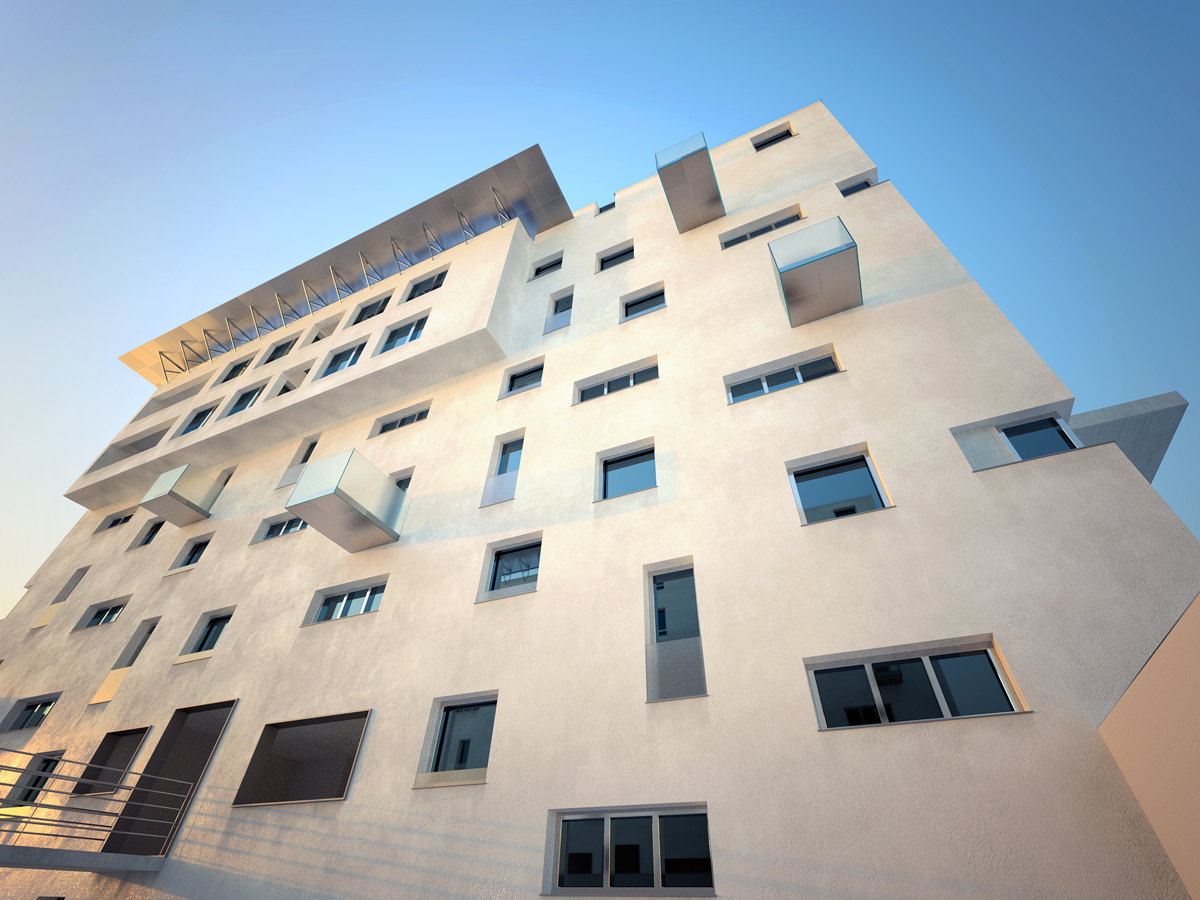
\includegraphics[width=6cm]{gfx/realistic01.jpg}
	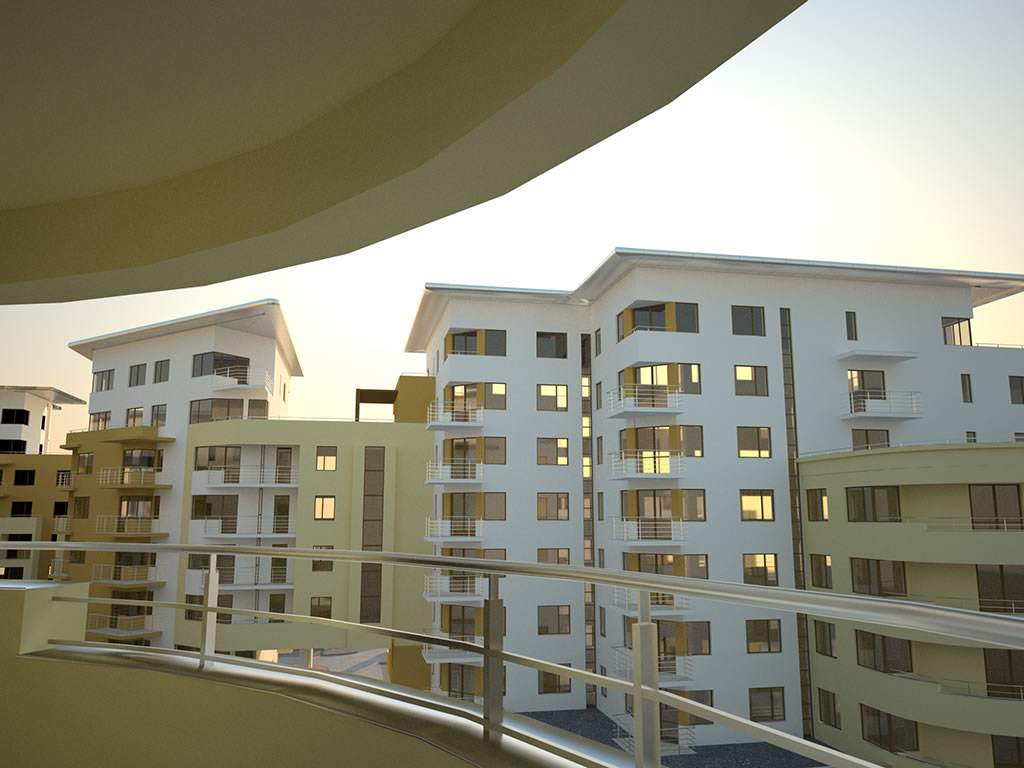
\includegraphics[width=6cm]{gfx/realistic03.jpg}
	\caption{Renderings done with Maxwell Renderer}
	\label{FIG-REALISTIC}
\end{figure}

Architects would benefit from a multimodal, non strict modeling system
for drafting in 3D and expose their ideas for clients to clients view, navigate
and criticize those drafts. For this to happen the desired solution must be:

\begin{itemize}
	\item a {\bf sketch board for architects} -- who can create and edit buildings and their features;
	\item a {\bf virtual urban scenery} for anyone -- therefore with a gentle learning curve, suitable for showcasing and reviewing architectural designs.
\end{itemize}

% families of problems
Building such a system involves solving the following problems:
\begin{itemize}
	\item Finding and sticking to a useful representation for urban scenery;
	\item Offering proper input interface for the users;
	\item Allowing a simple way of sketching geometry with easy learning curve;
	\item Aiding the user via suggestions and a fluid and efficient transforms;
	\item Navigation interface.
\end{itemize}


% navigation, +/-
One must be able to understand the world representation, navigate it and create or modify its contents.
In order to be immersed in the world, the interface should be larger than a regular computer screen
and proportions of the structural elements should be kept/suggested.
User input has to be based on devices that give him more expressiveness and allow human error,
preferably helping him out in subjects where a machine works better than humans do,
such as figuring out parallels or calculating areas.


% opensg/goggles/wall, etc
\subsection{Viewing Interface}
We aim at producing an immersive experience for a user or a small group of users.
How can that be accomplished, having to get user input at the same time?


% city representations
\subsection{Representing Urban Scenery}
A building can be as detailed as we want it to be.
Ideally, the architectural creations are surrounded by the environment
where they'll be built. So the system must be robust and enough to represent a city block.
How can we address the complexity of rendering a city?


% laser, motion, speech, gestures, smart widgets
\subsection{Getting User Input}
What are the viable alternatives to standard keyboard/mouse interaction with these objectives in mind?
How can a user sketch his ideas, give orders, navigate? Should users move, point, talk?


% sketching
\subsection{Sketching for Geometry Creation and Editing}
Given sketching input, how can the system interpret the sketch and reason an object out of it?
Should the process be iterative or all in one step?
How permissive should it be to irregular shapes?
 

% sketches in user space
\subsection{Helping the User: Suggested Constraints}
There's a subset of geometry that appears quite often in buildings.
The walls are generally box shaped, as are most windows. We often use concepts of symmetry,
the golden ratio, equilateral triangles, spherical structures such as domes, etc.

It would be of great use if while sketching one could be aided in keeping the ratio of
a rectangle, draw parallel or perpendicular lines, do extrusions and lathes.

What are the available ways by which one could be aided in these tasks?
How should the computer present reasoned content and replace inaccurate user content?
Users are very sensitive to losing control of applications.


% navigation
\subsection{Navigation}
By what means should the user convey his position and orientation in the world?
What can he do and how can he move?
How to avoid users getting lost in the virtual world?
